\documentclass[conference]{IEEEtran}
\usepackage[english]{babel}
\usepackage[usenames,dvipsnames]{color}
\usepackage{amssymb}
\usepackage{amsmath}
\usepackage{cases}
\usepackage{url}
% \usepackage[mathscr]{euscript}
\usepackage{mathrsfs}
\usepackage{multirow}
\usepackage{booktabs}

\usepackage[maxnames=10, sorting=none]{biblatex}
\renewcommand*{\bibfont}{\scriptsize}

\makeatletter
\let\oldsection=\section
\newcommand{\oldsectionStar}[1]{\oldsection*{#1}}
\newcommand{\oldsectionStarless}[1]{\oldsection{#1}}
\renewcommand{\section}{\@ifstar\oldsectionStar\oldsectionStarless}

\let\oldsubsection=\subsection
\renewcommand{\subsection}[1]{\oldsubsection{#1}}
\makeatother

% ---- Text
\linespread{0.9}
\topmargin -60pt
\textheight 750pt

\definecolor{ipurple}{RGB}{195,0,191}
\newcommand{\note}[1]{{\color{ipurple}$\star$}\marginpar{\scriptsize\color{ipurple}#1}}

% ---- Tables
\setlength{\topsep}{0pt}
\setlength{\abovecaptionskip}{2pt}
\setlength{\belowcaptionskip}{0pt}

% ---- Formulas
\setlength\abovedisplayskip{5pt}
\setlength\belowdisplayskip{5pt}

% ---- References
\newcommand{\eref}[1]{Eq.~(\ref{equ:#1})}
\newcommand{\sref}[1]{Sec.~\ref{sec:#1}}
\newcommand{\tref}[1]{Tab.~\ref{tab:#1}}

\newcommand{\elabel}[1]{\label{equ:#1}}
\newcommand{\slabel}[1]{\label{sec:#1}}
\newcommand{\tlabel}[1]{\label{tab:#1}}

% Basic mathematics
\newcommand{\idot}{\cdot}
\newcommand{\eqdef}{\stackrel{\text{\tiny def}}{=}}
\newcommand{\ifrac}[2]{{{#1}/{#2}}}
\newcommand{\bigo}{\mathcal{O}}

% ---- Spaces
\renewcommand{\L}[1]{\mathcal{L}_{#1}}

% ---- Sets
\newcommand{\real}{\mathbb{R}}
\renewcommand{\natural}[1]{\mathbb{N}_{#1}}

% ---- Matrices
\newcommand{\mtx}[1]{(#1)}
\newcommand{\m}[1]{\mathbf{\MakeUppercase{#1}}}

\newcommand{\mI}{\m{I}}
\newcommand{\mZero}{\m{0}}

\newcommand{\diag}[1]{\text{diag}\left(#1\right)}

% ---- Vectors
\renewcommand{\vec}[1]{(#1)^T}
\let\vtick\v
\renewcommand{\v}[1]{\mathbf{#1}}

\newcommand{\vZero}{\v{0}}

% Probability theory
\newcommand{\outcomes}{\Omega}
\renewcommand{\o}{\omega}
\newcommand{\sAlgebra}{\mathscr{F}}
\newcommand{\pMeasure}{\mathscr{P}}

\newcommand{\rv}[1]{\MakeUppercase{#1}}
\newcommand{\mrv}[1]{\mathbf{\MakeUppercase{#1}}}

\renewcommand{\exp}{\mu}
\newcommand{\var}{\sigma^2}
\newcommand{\std}{\sigma}

\newcommand{\vExp}{{\boldsymbol\mu}}
\newcommand{\mCov}{\m{\Sigma}}

\newcommand{\oExp}[1]{\mathbb{E}\left[#1\right]}
\newcommand{\oVar}[1]{\mathbb{V}\text{ar}\left[#1\right]}
\newcommand{\oCov}[1]{\mathbb{C}\text{ov}\left[#1\right]}
\newcommand{\oCorr}[1]{\mathbb{C}\text{orr}\left[#1\right]}

\newcommand{\PDF}{\rho}

\renewcommand{\rv}{RV}
\newcommand{\rvs}{RVs}

% ---- Normal distribution
\newcommand{\normal}[2]{\mathcal{N}\left( #1, #2 \right)}

% Thermal model
\newcommand{\system}{\mathcal{S}}

% ---- Time
\renewcommand{\t}{t}
\newcommand{\dt}{\Delta \t}
\newcommand{\period}{\mathcal{T}}
\newcommand{\sTime}{\mathcal{T}}

% ---- Temperature
\newcommand{\T}{\Theta}
\newcommand{\vTI}{\v{\tilde{X}}} % Internal temperature
\newcommand{\vTO}{{\boldsymbol\Theta}} % Output temperature
\newcommand{\mTO}{{\boldsymbol\Theta}}

\newcommand{\amb}{\text{amb}}

% ---- Power
\newcommand{\vP}{\v{P}}
\newcommand{\mP}{\m{P}}

\newcommand{\dyn}{\text{dyn}}
\newcommand{\leak}{\text{leak}}

\newcommand{\f}{\mathcal{F}}

% ---- Capacitance and conductance
\newcommand{\mC}{\m{C}}
\newcommand{\mG}{\m{G}}

% ---- Processor elements/thermal nodes mapping
\newcommand{\mM}{\m{\tilde{B}}}

% ---- Profiles
\newcommand{\part}{\boldsymbol{\Delta}}
\newcommand{\prof}[1]{\Pi\left[\part, #1\right]}

% ---- Differential-algebraic system
% dx/dt = A * x + B * u
% y = B^T * x
\newcommand{\vX}{\v{X}}
\newcommand{\mA}{\m{A}}
\newcommand{\mB}{\m{B}}

\newcommand{\mE}{\m{E}}
\newcommand{\mD}{\m{D}}

% Polynomial Chaos
\newcommand{\support}{S}
\newcommand{\pcb}{\Phi}
\newcommand{\pcn}{\gamma}
\newcommand{\pcc}[1]{\hat{#1}}
\newcommand{\oPC}[3]{\mathcal{P}_{#1}^{#2}\left[#3\right]}

\makeatletter
\def\oInner#1{\@ifnextchar\bgroup{\oInnerDouble{#1}}{\oInnerSingle{#1}}}
\def\oInnerSingle#1{\left\langle #1 \right\rangle}
\def\oInnerDouble#1#2{\oInnerSingle{#1, #2}}
\makeatother

% ---- Integration
\newcommand{\qdn}[1]{\hat{#1}}
\newcommand{\qdw}{w}
\newcommand{\oQuad}[3]{\mathcal{Q}_{#1}^{#2}\left[#3\right]}

% Uncertain parameters
% ---- Correlated
\newcommand{\U}{U}
\newcommand{\vU}{\v{U}}

% ---- Independent
\newcommand{\Z}{Z}
\newcommand{\vZ}{\v{Z}}
\newcommand{\vz}{\boldsymbol{\zeta}}

\newcommand{\oTransform}[1]{T\left[#1\right]}
\newcommand{\oInvTransform}[1]{T^{-1}\left[#1\right]}

% ---- Process variation
\newcommand{\Leff}{L}
\newcommand{\nLeff}{L}
\newcommand{\gLeff}{{L^{(g)}}}
\newcommand{\lLeff}{L^{(l)}}
\newcommand{\Lth}{\lambda_\text{th}}
\newcommand{\corrLength}{\eta}

% Indexes
\newcommand{\nodes}{N_\text{n}}
\newcommand{\cores}{{N_\text{p}}}
\newcommand{\steps}{N_\text{s}}
\newcommand{\vars}{{N_\text{v}}}

\newcommand{\pcorder}{{N_\text{po}}}
\newcommand{\pcterms}{{N_\text{pt}}}

\newcommand{\qdlevel}{N_\text{ql}}
\newcommand{\qdorder}{N_\text{qo}}
\newcommand{\qdorderone}{\tilde{N}_\text{qo}}
\newcommand{\qdprecision}{N_\text{qp}}

\newcommand{\mcsamples}{N_\text{mcs}}

% Experimental results
\newcommand{\hostOS}{OS X 10.8}
\newcommand{\hostHardware}{a MacBook Pro 6.2 with Intel Core i7 2.66 GHz and 8 GB of RAM}
% \newcommand{\hostOS}{a GNU/Linux distribution}
% \newcommand{\hostHardware}{Intel Core i7 3.4 GHz with 8 GB of RAM}

\newcommand{\eExp}{\err{\mathbb{E}}}
\newcommand{\eVar}{\err{\mathbb{V}\text{ar}}}
\newcommand{\ePDF}{\err{\PDF}}

\newcommand{\err}[1]{\delta#1}

\newcommand{\mcs}[1]{\scriptstyle \mcsamples = 10^#1}
\newcommand{\csep}{\hspace{7pt}}
\newcommand{\psep}{\hspace{15pt}}


\bibliography{include/references.bib}

\begin{document}
  \title{Stochastic Temperature Analysis of\\Multiprocessor Systems}

  \author{
    \IEEEauthorblockN{Ivan Ukhov}
    \IEEEauthorblockA{Link\"{o}ping University\\Sweden\\ivan.ukhov@liu.se}
    \and
    \IEEEauthorblockN{Petru Eles}
    \IEEEauthorblockA{Link\"{o}ping University\\Sweden\\petru.eles@liu.se}
    \and
    \IEEEauthorblockN{Zebo Peng}
    \IEEEauthorblockA{Link\"{o}ping University\\Sweden\\zebo.peng@liu.se}
  }

  \maketitle

  \begin{abstract}
    Temperature is important.
  \end{abstract}

  \section{Introduction} \slabel{introduction}
  The variations in the dynamic power due to the process variation are negligible whereas the leakage power is the major headache of the designer \cite{juan2012, srivastava2010}.

It is widely accepted that the leakage current has a log-normal distribution, cf. \cite{juan2012, srivastava2010}. The sub-threshold leakage is the most sensible to the process variation while the gate leakage has become less important with the introduction of high-k dielectrics \cite{juan2012}.

The most commonly used approach to perform the \sta\ is Monte Carlo sampling (MCS) techniques coupled with a deterministic thermal simulator. The problem is in the low rate of convergence, e.g., the mean value converges as $1/\sqrt{n}$ where $n$ is the number of simulations \cite{xiu2009}. Therefore, the MCS requires an unaffordably large number of realizations of the system to be performed.

In this work, we use a mathematical framework called the generalized polynomial chaos (gPC), which is the current state-of-the-art of numerical analysis of stochastic systems \cite{xiu2009, xiu2002}. The core of the gPC is the decomposition of stochastic processes into infinite sums of orthogonal polynomials of random variables (r.v.'s) that significantly eases the subsequent analysis. As its name suggests, the gPC is a generalization of the original polynomial chaos (PC) where only Hermite polynomials and Gaussian r.v.'s were considered \cite{ghanem1991}. In contrast, the gPC employs a broad family of orthogonal polynomials from the Askey scheme, which the Hermite polynomials are a subset of, and handles different probability distributions. It can be shown that \emph{any} functional with a finite variance can be approximated with a PC/gPC expansion, and this expansion converges in the $\L{2}$ (mean-square) sense.

In \cite{shen2009}, the PC is applied to estimate the full-chip leakage current.

The output of the proposed framework constitutes the stochastic power profile of the multiprocessor system and the corresponding stochastic temperature profile.

A possible way to speed up the analysis is to employ the model-order reduction (MOR) techniques \cite{benner2011}, which can dramatically decrease the number of state variables of the system. These techniques can be considered as a preprocessing step and, therefore, they are applicable to all the above-mentioned methods.

The rest of the paper is organazed as follows.


  \section{Preliminaries}
  \subsection{Conventional Notations}
Throughout this article, we use the following notations. $\real$ is the set of real number and $\natural{n}$ is the set of integers greater or equal to $n$. Boldface letters denote vectors and matrices, e.g., $\m{M} = \mtx{m_{ij}} \in \real^{n \times m}$ denotes a $n \times m$ real matrix, and $\v{V} = \vec{v_i} \in \real^n$ denotes and an $n$-dimensional real column vector. $\m{M}^T$ and $e^\m{M}$ are the transpose and matrix exponential of $\m{M}$, respectively. $\diag{m_i} \in \real^{n \times n}$ denotes a $n \times n$ diagonal matrix. $\mI_n$ is the $n \times n$ identity matrix, and $\mZ_{n \times m}$ is the $n \times m$ zero matrix; we shall omit these indexes when the actual dimensions of $\mI$ and $\mZ$ are clear from the context.

\subsection{Elements of Probability Theory}
Let $(\outcomes, \sAlgebra, \pMeasure)$ be a complete probability space \cite{durrett2010} where $\outcomes$ is a set of outcomes, $\sAlgebra \subset 2^\outcomes$ is a $\sigma$-algebra on $\outcomes$, and $\pMeasure: \sAlgebra \to [0, 1]$ is a probability measure induced on the measurable space $(\outcomes, \sAlgebra)$. A $\sAlgebra$-measurable function $\rv{X}(\o): \outcomes \to \real$ is called a \definition{random variable} (r.v.). Denote $\exp_\rv{X} = \oExp{\rv{X}(\o)}$ the expectation of $\rv{X}(\o)$ and $\var_\rv{X} = \oVar{\rv{X}(\o)}$ its variance. A $\pMeasure$-measurable, vector-valued function $\mrv{X}(\o): \outcomes \to \real^n$ is called a multivariate random variable (m.r.v.) with $\vExp_\mrv{X} = \oExp{\mrv{X}(\o)}$ and $\mCov_\mrv{X} = \oCov{\mrv{X}(\o)}$ being its expectation vector and covariance matrix, respectively. A \definition{stochastic process} is a parametrized collection of r.v.'s $\{ \rv{X}(\o, \t) \}_{\t \in \sTime}$ where $\sTime$ is a parameter space, which is usually assumed to be the real half line $[0, \infty)$ meaning time. $\{ \mrv{X}(\o, \t) \}_{\t \in \sTime}$ denotes a $n$-dimensional stochastic process. We shall omit the argument $\o \in \outcomes$ when the stochastic nature of the quantity under consideration is clear from the context.

The covariance matrix is necessarily a real, symmetric matrix. Therefore, it admits the eigenvalue factorization \cite{press2007} in the form $\mCov_\mrv{X} = \m{V}_{\mCov_\mrv{X}} \m{\Lambda}_{\mCov_\mrv{X}} \m{V}_{\mCov_\mrv{X}}^T$ where $\m{V}_{\mCov_\mrv{X}}$ and $\m{\Lambda}_{\mCov_\mrv{X}}$ are an orthogonal matrix of the eigenvectors and a diagonal matrix of the eigenvalues of $\mCov_\mrv{X}$, respectively. Denote $\oEigen{\mCov_\mrv{X}} = \m{V}_{\mCov_\mrv{X}} {\m{\Lambda}_{\mCov_\mrv{X}}}^\ifrac{1}{2}$. In this notation, $\mCov_\mrv{X} = \oEigen{\mCov_\mrv{X}} \oEigen{\mCov_\mrv{X}}^T$. Consequently, $\mrv{X}$ can be normalized as $\mrv{X} = \oEigen{\mCov_\mrv{X}} \mrv{y} + \vExp_\mrv{X}$ where $\oExp{\mrv{y}} = \mZ$ and $\oCov{\mrv{y}} = \mI$.

\subsection{Architecture Model} \slabel{architecture-model} \slabel{system-profiles}
Consider a multiprocessor platform that comprises $\cores$ processing elements of any kind and is equipped with a thermal package. Let $\system$ be a \definition{high-level description} of the platform that includes the following information:
\begin{itemize}
  \item The floorplan of the die (the location and dimensions of the processing elements). In the case of 3D ICs, the floorplans of each of the stacked chips.
  \item The configuration of the thermal package (the dimensions of each of the layers).
  \item The thermal parameters of the materials that the die and package are made of (the thermal conductivity, specific heat, convection capacitance, and convection resistance).
\end{itemize}

Suppose the given system depends on a number of \definition{uncertain parameters}, i.e., r.v.'s that are possibly correlated. Let $(\outcomes, \sAlgebra, \pMeasure)$ be the corresponding probability space and $\vU(\o) = \vec{\param_i(\o)} \in \real^\vars$, $\o \in \outcomes$, be a $\vars$-dimensional vector of these parameters. In this work, we assume that the uncertainties $\vU(\o)$, $\o \in \outcomes$, are a result of the process variation and manifest themselves in the deviation of the actual power dissipation of the system from the nominal value (see \sref{power-model}). In this case, $\outcomes$ represents the outcomes of the manufacturing process, which the given multiprocessor system is a product of. For brevity, we shall not write explicitly the dependency on $\vU(\o)$ and use $\o$ instead, i.e., $f(\o)$ should be understood as $f(\vU(\o))$.

Let $\prof{\m{Q}}$ be a \definition{system profile} of a quantity $Q$ over a time interval $\period$ where $\part = \{ 0 = \t_1 < \dotsc < \t_{\steps + 1} = \period \}$ is a partition of $\period$ into $\steps$ subintervals $\{ \dt_i = \t_{i+1} - \t_i \}_{i = 1}^{\steps}$, and $\m{Q} \in \real^{\cores \times \steps}$ is a matrix that captures the values of $Q$ for all $\cores$ processing elements at all $\steps$ time intervals. In particular, we are interested in the power and temperature profiles denoted by $\prof{\mP}$ and $\prof{\mTO}$, respectively (hereafter, $P$ stands for power and $\Theta$ for temperature). Since the system under consideration is affected by the process variation, we make a distinction between deterministic (nominal) or stochastic power and temperature profiles. In the stochastic case, each column of a system profiles is a m.r.v. with a known multivariate probability distribution.


  \section{Problem Formulation} \slabel{problem-formulation}
  The total dissipation of power is composed of two major parts: dynamic and static.
The influence of process variation on the dynamic power is known to be negligibly small \cite{srivastava2010}; on the other hand, the variability of the static power is substantial, in which the subthreshold leakage current contributes the most \cite{juan2011, juan2012}.
Hence, we shall focus on the subthreshold leakage and, more specifically, on the effective channel length, denoted by $\Leff$, since it has the strongest influence on leakage and is severely deteriorated by process variation \cite{chandrakasan2001}.
In particular, $\Leff$ also affects the threshold voltage \cite{juan2011}.

It is well known that the dispersion due to process variation of the effective channel length around the nominal value resembles a bell shape, which is similar to the ones owned by Gaussian distributions.
Therefore, such variations are often conveniently modeled using Gaussian variables \cite{srivastava2010, juan2011, juan2012, chandra2010, huang2009, lee2013, shen2009, bhardwaj2006, ghanta2006}.
In this work, due to both the underlying physics and demonstration purposes, we make a step further and bake right into the model the fact that the effective channel length---occupying the space between the drain and source of a nanoscopic transistor---cannot be arbitrarily large or take a negative value, as Gaussian distributions allow it to do.
In other words, we require the model of $\Leff$ to have a bounded support.
With this in mind, we propose to model physically-bounded parameters using the four-parametric family of beta distributions: $\dBeta(a, b, c, d)$ where $a$ and $b$ are the shape parameters, and $c$ and $d$ are the left and right bounds of the support, respectively.
$a$ and $b$ can be chosen in such a way that the typically found bell shape of the distribution is preserved.
An illustration is given in \fref{beta-normal} where we fitted a beta distribution to the standard Gaussian distribution.\footnote{Alternatively, one can match the moments of the distributions.}
It can be seen that the curves are nearly indistinguishable, but the beta one has a bounded support $[-4, 4]$, which can potentially lead to more realistic models.

\begin{figure}[t]
  \centering
  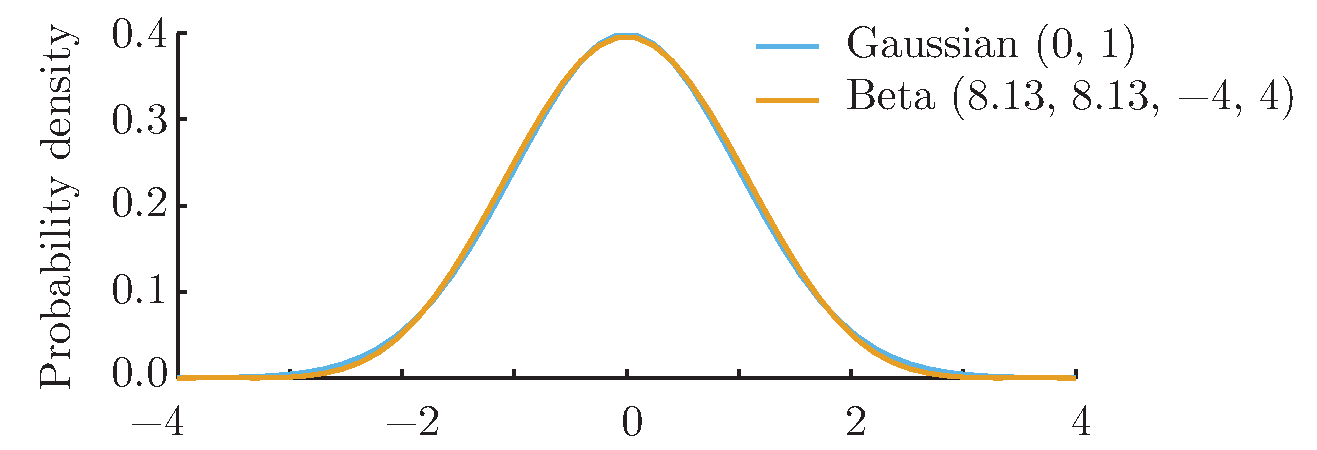
\includegraphics[width=0.9\ColumnWidth]{include/assets/beta-normal.pdf}
  \caption{The standard Gaussian distribution and a fitted beta distribution.}
  \flabel{beta-normal}
\end{figure}

The variability of $\Leff$ is split into global $\gLeff$ and local $\lLeff$ parts \cite{chandra2010, shen2009}.\footnote{Without loss of generality, $\gLeff$ can be treated as a composition of independent inter-lot, inter-wafer, and inter-die variations; likewise, $\lLeff$ can be treated as a composition of independent and dependent local variations.}
$\gLeff$ is assumed to be shared among all processing elements whereas each processing element has its own local parameter $\lLeff_i$.
Therefore, the effective channel length the $i$th processing element is modeled as follows:
\begin{equation} \elabel{leakage-partition}
  \Leff_i = \nLeff + \gLeff + \lLeff_i
\end{equation}
where $\nLeff$ is the nominal value of the effective channel length.
Hence, the uncertain parameters of the problem are
\begin{equation} \elabel{uncertain-parameters}
  \vU = \vec{\lLeff_1, \dotsc, \lLeff_\nprocs, \gLeff}.
\end{equation}

Global variations are typically assumed to be uncorrelated with respect to the local ones.
The latter, however, are known to have high spatial correlations, which we shall model using the following correlation function:
\begin{equation} \elabel{correlation-function}
  \fCorr(\vR_i, \vR_j) = \eta \; \fCorrSE(\vR_i, \vR_j) + (1 - \eta) \fCorrOU(\vR_i, \vR_j)
\end{equation}
where $\vR_i \in \real^2$ is the spatial location of the center of the $i$th processing element relative to the center of the die. The correlation function is a composition of two kernels:
\begin{align*}
  & \fCorrSE(\vR_i, \vR_j) = \exp\left(- \frac{\norm{\vR_i - \vR_j}^2}{\lCorrSE^2} \right) \text{ and} \\
  & \fCorrOU(\vR_i, \vR_j) = \exp\left(- \frac{\abs{\,\norm{\vR_i} - \norm{\vR_j}\,}}{\lCorrOU} \right),
\end{align*}
which are known as the squared-exponential and Ornstein-Uhlenbeck kernels, respectively.
$\eta \in [0, 1]$ is a weight coefficient balancing the kernels; $\lCorrSE$ and $\lCorrOU > 0$ are so-called length-scale parameters; and $\norm{\cdot}$ stands for the Euclidean distance.
The choice of the correlation function in \eref{correlation-function} is guided by the observations of the correlations induced by the fabrication process \cite{chandrakasan2001, friedberg2005, cheng2011}: $\fCorrSE$ imposes similarities between the spatial locations that are close to each other, and $\fCorrOU$ imposes similarities between the locations that are at the same distance from the center of the die (see also \cite{huang2009, ghanem1991, lee2013, bhardwaj2008, ghanta2006}).
The length-scale parameters $\lCorrSE$ and $\lCorrOU$ control the extend of these similarities, \ie, the range wherein the influence of one point on another is significant.

Although \eref{correlation-function} captures certain features inherent to the fabrication process, it is still an idealization.
In practice, it can be difficult to make a justifiable choice and tune such a formula, which is a prerequisite for the techniques in \sref{prior-work} based on the (continuous) KL decomposition.
A correlation matrix, on the other hand, can readily be estimated from measurements and, thus, is a more probable input to PTA.
Thus, we use \eref{correlation-function} with the only purpose of constructing a correlation matrix of $\{ \lLeff_i \}$.
For convenience, the resulting matrix is extended by one dimension to pack $\gLeff$ and $\{ \lLeff_i \}$ together.
In this case, the correlation matrix obtains one additional non-zero element on the diagonal.
Taking into account the variances of the variable, the final covariance matrix of the whole random vector $\vU$ (see \eref{uncertain-parameters}) is formed, which we denote by $\mCov_\vU$.

To conclude, an input to our analysis is the marginal distributions of the parameters $\vU$, which are beta distributions, and the corresponding covariance matrix $\mCov_\vU$.


  \section{Proposed Framework}
  In this section, we present the proposed framework step by step and begin with preprocessing of the input parameters.

\subsection{Uncertain Parameters} \slabel{uncertain-parameters}
The total dissipation of power is composed of two major parts: dynamic and leakage. The influence of process variation on the dynamic power is known to be negligibly small \cite{juan2011, juan2012, srivastava2010}; on the other hand, the variability of leakage is substantial, wherein the subthreshold current contributes the most \cite{juan2011, juan2012}. Hence, we focus on the subthreshold leakage and, more specifically, on the effective channel length denoted by $\Leff$. The variations of $\Leff$ are split into global (inter-die) and local (intra-die) parts \cite{chandra2010, juan2011, juan2012, srivastava2010, shen2009}. The global contribution is shared among all the processing elements and, therefore, is modeled as a single \rv\ $\gLeff(\o)$; furthermore, $\gLeff(\o)$ is typically assumed to be independent with respect to the local variations. The latter, however, are known to have high spatial correlations, which, due to particularities of the manufacturing process, often bear radial structures \cite{friedberg2005, cheng2011}. Therefore, as in \cite{ghanta2006}, we model the intra-die variations as a continuous-space stochastic process $\lLeff(r, \o)$ with the following radial covariance function \cite{ghanem1991}:
\begin{equation} \elabel{covariance-function}
  \fCov{\lLeff}{r_i, r_j} = e^{-|r_i - r_j|/\corrLength}
\end{equation}
where $r_i$ is the distance from the $i$th processing element to the center of the die, and $\corrLength$ is the correlation length. In words, the structure implies that the smaller the radial distance between two processing elements on the die, the more likely they are to have similar deviations of the effective channel length. Finally, it is generally accepted that the variations of the channel length have Gaussian distributions \cite{juan2011, juan2012, srivastava2010}. Therefore, we assume that the \rv\ $\gLeff(\o)$ as well as the process $\lLeff(r, \o)$ are Gaussian.

$\gLeff(\o)$ and $\lLeff(r, \o)$ form the input set of uncertain parameters $\vU(r, \o)$, which is to be processed in order to extract a finite set of mutually independent \rvs\ $\vZ(\o)$. Following the guidelines in \sref{uncertain-parameters}, Stage~1, the KL expansion suits the best in such a situation. A thorough elaboration on KL is out of the scope of this paper; however, the interested reader is referred to \aref{uncertain-parameters} where KL is applied to \eref{covariance-function}.


\subsection{Power Model} \slabel{power-model}
The (total) power dissipation of the system with $\cores$ processing elements is given as the following sum:
\begin{equation} \elabel{power-model}
  \vP(\t, \o) = f_\dyn(\vP_\dyn(\t), \o) + f_\leak(\vTO(\t, \o), \o)
\end{equation}
where $f_\dyn, f_\leak: \real^\cores \times \outcomes \to \real^\cores$ model the dynamic and leakage power, respectively, as functions of the uncertain parameters $\vZ(\o)$. In addition, $f_\dyn$ depends on the nominal dynamic power $\vP_\dyn \in \real^\cores$, and the leakage part, $f_\leak$, depends on the operating temperature $\vTO \in \real^\cores$ due to the well-known non-linear interdependency between leakage and temperature, c.f. \cite{srivastava2010, liu2007}. We do not impose any further restrictions on $f_\dyn$ and $f_\leak$, and let the user to decide\footnote{One can easily find a dicent number of alternatives in the contemporary literature, for instance, follow the reference in \cite{srivastava2010}.}. Moreover, the functions are not required to have explicit mathematical formulations; they can be given as a `black box' as long as its inputs are in the set $\{ \vP_\dyn, \vTO, \vZ \}$.


\subsection{Thermal Model} \slabel{thermal-model}
In this section, we provide additional details on the thermal model utilized by the proposed framework at \stage{3}\ described in \sref{thermal-model}.
We use the widespread model based on Fourier's heat equation \cite{skadron2004}, which, after a proper spacial discretization, leads to the following system:
\begin{subnumcases}{\elabel{fourier-system-original}}
  \mC \: \frac{d\,\vTI(\t)}{d\t} + \mG \: \vTI(\t) = \mM \: \vP(\t) \elabel{fourier-original} \\
  \vTO(\t) = \mM^T \vTI(\t) + \vTO_\amb
\end{subnumcases}
where the number of differential equations is equal to the number of thermal nodes denoted by $\nnodes$; $\mC \in \real^{\nnodes \times \nnodes}$ and $\mG \in \real^{\nnodes \times \nnodes}$ are a diagonal matrix of the thermal capacitance and a symmetric, positive-definite matrix of the thermal conductance, respectively; $\vTI \in \real^\nnodes$ is a vector of the difference between the temperature of the thermal nodes and the ambient temperature; $\vP \in \real^\nprocs$ and $\mM \in \real^{\nnodes \times \nprocs}$ are a vector of the power dissipation of the processing elements and its mapping to the thermal nodes, respectively; $\vTO \in \real^\nprocs$ is a vector of the temperature of the processing elements; and $\vTO_\amb \in \real^\nprocs$ is a vector of the ambient temperature.
$\mM$ distributes power across the thermal nodes.
Assuming that one processing element is mapped onto one thermal node, $\mM$ is filled in with zeros except for $\nprocs$ elements equal to unity that are located on the main diagonal.
For convenience, we perform an auxiliary transformation of the system in \eref{fourier-system-original} using \cite{ukhov2012}
\[
  \vS = \mC^\frac{1}{2} \vTI, \hspace{1em} \mA = -\mC^{-\frac{1}{2}} \mG \mC^{-\frac{1}{2}}, \hspace{1em} \text{and} \hspace{1em} \mB = \mC^{-\frac{1}{2}} \mM
\]
and obtain the system in \eref{fourier-system} where the coefficient matrix $\mA$ preserves the symmetry and positive-definiteness of $\mG$.
In general, the differential part in \eref{fourier-system-original} (and in \eref{fourier-system}) is nonlinear due to the source term $\vP(\t)$ since we do not make any assumptions about its structure (see the discussion in \sref{power-model}).
Therefore, there is no closed-form solution to the system.

The time intervals of the power and temperature profiles are assumed to be short enough such that the total power of a processing element can be approximated by a constant within one interval.
In this case, \eref{fourier-original} (and \eref{fourier-de}) is a system of linear differential equations that can be solved analytically.
The solution is as follows \cite{ukhov2012}:
\begin{equation} \elabel{ode-solution}
  \vS(\t) = \mCF(\t) \: \vS(0) + \mCS(\t) \: \vP(0)
\end{equation}
where $\t$ is restricted to one time interval, $\vP(0)$ is the power dissipation at the beginning of the time interval with respect to the corresponding temperature,
\begin{align*}
  & \mCF(\t) = e^{\mA \t} \in \real^{\nnodes \times \nnodes}, \hspace{1em} \text{and} \\
  & \mCS(\t) = \mA^{-1} (e^{\mA \t} - \mI) \: \mB \in \real^{\nnodes \times \nprocs}.
\end{align*}
The procedure is to be repeated for all $\nsteps$ time intervals starting from the initial temperature, which, without loss of generality, is assumed to be equal to the ambient temperature.
Note that, when the power profile is evenly sampled, the coefficient matrices $\mCF(\t)$ and $\mCS(\t)$ are constant and can be efficiently computed using the technique in \cite{ukhov2012}.
It is also worth noting that the described solution method belongs to the family of so-called exponential integrators, which have good stability properties; refer to \cite{hochbruck2010} for an overview.
Finally, taking into account $\vU$, we obtain \eref{recurrence}, operating on stochastic quantities.


\subsection{Polynomial Chaos Expansion} \slabel{polynomial-chaos}
At \stage{4}, the independent \rvs, power model, and thermal model are fused together under the desired workload, $\profilePdyn$, to produce the corresponding stochastic power $\profileP{\o}$ and temperature $\profileT{\o}$ profiles. The obtained stochastic profiles are nothing more than two polynomials of $\Z_1(\o)$ and $\Z_2(\o)$ with time-dependent coefficients.

The construction of PC expansions is based on the Hermite basis (see \tref{askey}) as it was found to be optimal in situations involving Gaussian parameters \cite{xiu2010}.
A one-dimensional example of the basis is given in \fref{hermite} where the first six Hermite polynomials $\{ \pcb_i(\z) \}_{i = 1}^6$ are displayed.

In two dimensions, assuming a second-total-order PC expansion, the temperature at the $k$th moment of time is
\begin{align*}
  \vTO_k(\o) &= \pccs_{k1} + \pccs_{k2} \Z_1(\o) + \pccs_{k3} \Z_2(\o) + \pccs_{k4} \Z_1(\o) \Z_2(\o) \\
  & \qquad \qquad {} + \pccs_{k5} (\Z_1(\o)^2 - 1) + \pccs_{k6} (\Z_2(\o)^2 - 1)
\end{align*}
where $\pccs_{ki}$ are vectors with two elements corresponding to the two processors.

Once the basis has been chosen, we need to compute the corresponding coefficients, specifically, $\pcc{\vP}_i$ in \eref{pc-expansion}. As shown in \aref{polynomial-chaos}, the computation of $\pcc{\vP}_i$ involves multidimensional integration with respect to the \pdf\ of the \rvs\ $\vZ(\o)$.
In numerical analysis, this task is typically accomplished by virtue of a quadrature rule \cite{press2007}, which, loosely speaking, is a weighted summation over the integrand values computed at prescribed points. A natural choice of a quadrature rule when the weight function is a Gaussian \pdf\ is the Gauss-Hermite quadrature. Further details are given in \aref{gauss-quadrature}.

To summarize, we have completed four out of five stages of the proposed UQ framework depicted in \fref{algorithm}. The result is a light surrogate of the model in \eref{fourier-system}. At each moment of time, the surrogate is composed of two $\nprocs$-valued polynomials, one for power and one for temperature, that are defined in terms of $\nvars$ mutually independent \rvs; an example of such a polynomial is given in \eref{pc-k}. The constructed representation can be trivially analyzed to retrieve various statistics of the system in \eref{fourier-system}, and this is \stage{5}\ in \fref{algorithm}, which will be illustrated as a part of the next section.

\begin{figure}
  \centering
  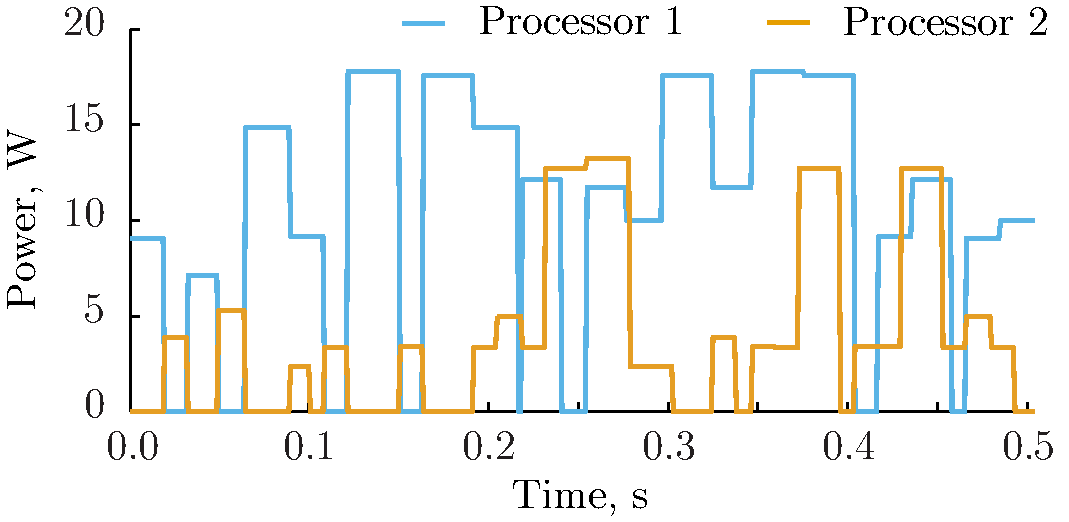
\includegraphics[width=1.00\columnwidth]{include/assets/application-power.pdf}
  \vspace{-0.5em}
  \caption{A dynamic power profile.}
  \flabel{application-power}
  \vspace{-0.5em}
\end{figure}

Assume that the dynamic power profile, $\profilePdyn$, corresponding to the considered workload is the one shown in \fref{application-power}.

\begin{figure}[bl]
  \vspace{-1.0em}
  \centering
  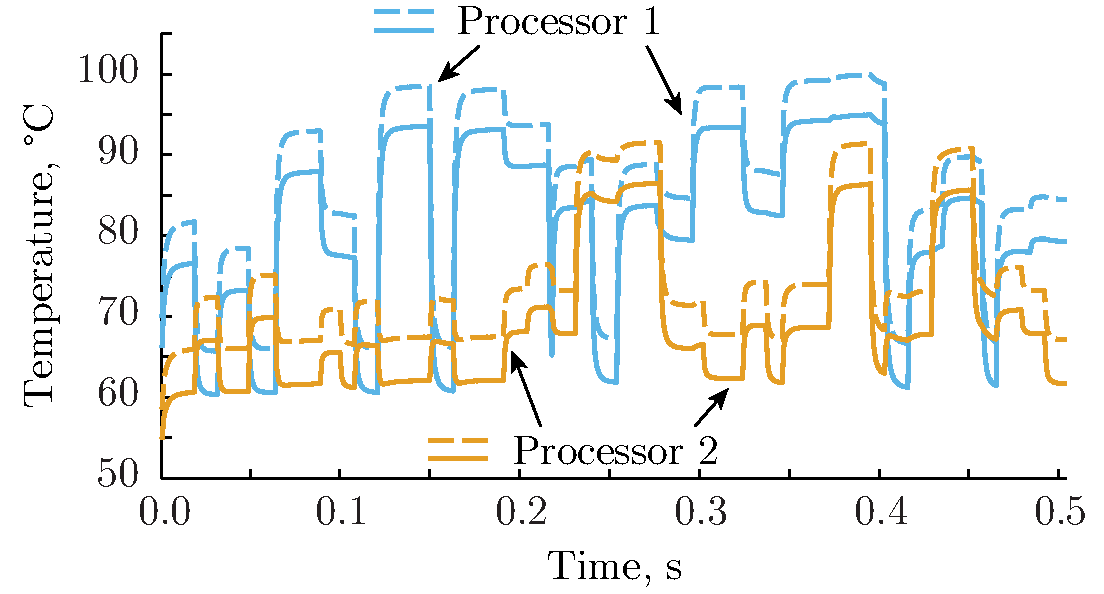
\includegraphics[width=0.90\columnwidth]{include/assets/application-temperature.pdf}
  \vspace{-0.5em}
  \caption{The expected temperature (the solid lines) and one standard deviation above it (the dashed lines).}
  \flabel{application-temperature}
\end{figure}

The expansion for power has the same structure but different coefficients.
Such a series might be shorter or longer depending on the accuracy requirements.
As we see, our surrogate model has a negligibly small computational cost to undertake UQ at \stage{5}: for any outcome of the uncertain parameters $\vZ(\o) \equiv \vZ$, we can easily compute the corresponding temperature by plugging $\vZ$ into the above equation; the same applies for power.
Thus, such characteristics as \cdfs\ and \pdfs\ (see \fref{motivation-pdf}) can be rigorously estimated. Furthermore, the expectation and variance at the $k$th moment of time are calculated as simply as
\[
  \oExp{\vTO_k(\o)} = \pccs_{k1} \hspace{1em} \text{and} \hspace{1em} \oVar{\vTO_k(\o)} = \sum_{i = 2}^{6} \pcn_i \: \pccs_{ki}^2
\]
where $\pcn_i$ are normalization constants, and the squaring should be understood element-wise.
For the nominal power profile $\profilePdyn$ depicted in \fref{application-power}, we obtain the corresponding stochastic temperature profile $\profileT{\o}$ and can observe, \eg, its expectation and standard deviation; they are plotted in \fref{application-temperature}.
The displayed curves closely match those obtained via MC simulations with $10^4$ samples; however, our method takes less than a second, on a personal laptop, while MC sampling takes more than a day, which we discuss in \sref{experimental-results}.


\subsection{Output Analysis}
For each time interval of the input dynamic power profile $\prof{\mP_\dyn}$, \eref{pc-recurrence} provides the coefficients of the PC expansion for temperature $\vTO(\t, \o)$ based on the coefficients of the PC expansion for power $\vP(\t, \o)$. Consequently, the output of the proposed framework constitutes two stochastic system profiles: the power $\prof{\mP(\o)}$ and temperature $\prof{\mTO(\o)}$ profiles. Due to orthogonality of the components of a PC expansion, the obtained traces can easily be analyzed from different perspectives \cite{eldred2009, maitre2010}. For instance, consider the PC expansion of temperature for the $k$th time interval
\begin{equation} \elabel{pc-k}
  \oPC{\vars}{\pcorder}{\vTO_k(\t, \o)} = \sum_{i = 1}^{\pcterms} \pcc{\vTO}_{ki}(\t) \pcb_i(\vZ(\o))
\end{equation}
where $\t \in [0, \dt_k]$, and $\pcc{\vTO}_{ki}(\t)$ are found using \eref{pc-recurrence} and \eref{fourier-output}. Let us, for example, find the expectation and covariance of the expansion. By definition \cite{xiu2002}, the first polynomial $\pcb_1(\vZ(\o))$ in a polynomial basis is 1, hence, $\oExp{\pcb_1(\vZ(\o))} = 1$. Therefore, using \eref{orthogonality}, we conclude that $\oExp{\pcb_i(\vZ(\o))} = 0$ for $i \in \{ 2, \dotsc, \pcterms \}$. Consequently, the expectation is
\[
  \oExp{\vTO_k(\t, \o)} = \pcc{\vTO}_{k1}(\t)
\]
and the covariance is
\[
  \oCov{\vTO_k(\t, \o)} = \sum_{i = 2}^{\pcterms} \pcc{\vTO}_{ki}(\t) \pcc{\vTO}_{ki}(\t)^T \pcn_i
\]
The probability density (or mass) function as well as the cumulative distribution function can be estimated by sampling \eref{pc-k}. Each sample is a trivial evaluation of a multivariate polynomial. On the contrary, when a MC-based technique is employed to quantify \eref{fourier-system}, a sample is a complete simulation of $\prof{\mP_\dyn}$. Since the number of such samples should be considerably large to obtain reliable results \cite{xiu2009}, MC-based approaches become highly time consuming.



  \section{Illustrative Example} \slabel{illustrative-example}
  So far we have not made any assumptions regarding the cause of the variability of the power term in the thermal system given by \eref{fourier-system}.
In this section, we shall consider a particular application of the proposed framework.
To this end, we begin with the problem formulation of this application.

The total dissipation of power is composed of two major parts: dynamic and static.
The influence of process variation on the dynamic power is known to be negligibly small \cite{srivastava2010}; on the other hand, the variability of the static power is substantial, in which the subthreshold leakage current contributes the most \cite{juan2011, juan2012}.
Hence, we shall focus on the subthreshold leakage and, more specifically, on the effective channel length, denoted by $\Leff$, since it has the strongest influence on leakage and is severely deteriorated by process variation \cite{chandrakasan2001}.
In particular, $\Leff$ also affects the threshold voltage \cite{juan2011}.

It is well known that the dispersion due to process variation of the effective channel length around the nominal value resembles a bell shape, which is similar to the ones owned by Gaussian distributions.
Therefore, such variations are often conveniently modeled using Gaussian variables \cite{srivastava2010, juan2011, juan2012, chandra2010, huang2009, lee2013, shen2009, bhardwaj2006, ghanta2006}.
In this work, due to both the underlying physics and demonstration purposes, we make a step further and bake right into the model the fact that the effective channel length---occupying the space between the drain and source of a nanoscopic transistor---cannot be arbitrarily large or take a negative value, as Gaussian distributions allow it to do.
In other words, we require the model of $\Leff$ to have a bounded support.
With this in mind, we propose to model physically-bounded parameters using the four-parametric family of beta distributions: $\dBeta(a, b, c, d)$ where $a$ and $b$ are the shape parameters, and $c$ and $d$ are the left and right bounds of the support, respectively.
$a$ and $b$ can be chosen in such a way that the typically found bell shape of the distribution is preserved.
An illustration is given in \fref{beta-normal} where we fitted a beta distribution to the standard Gaussian distribution.\footnote{Alternatively, one can match the moments of the distributions.}
It can be seen that the curves are nearly indistinguishable, but the beta one has a bounded support $[-4, 4]$, which can potentially lead to more realistic models.

\begin{figure}[t]
  \centering
  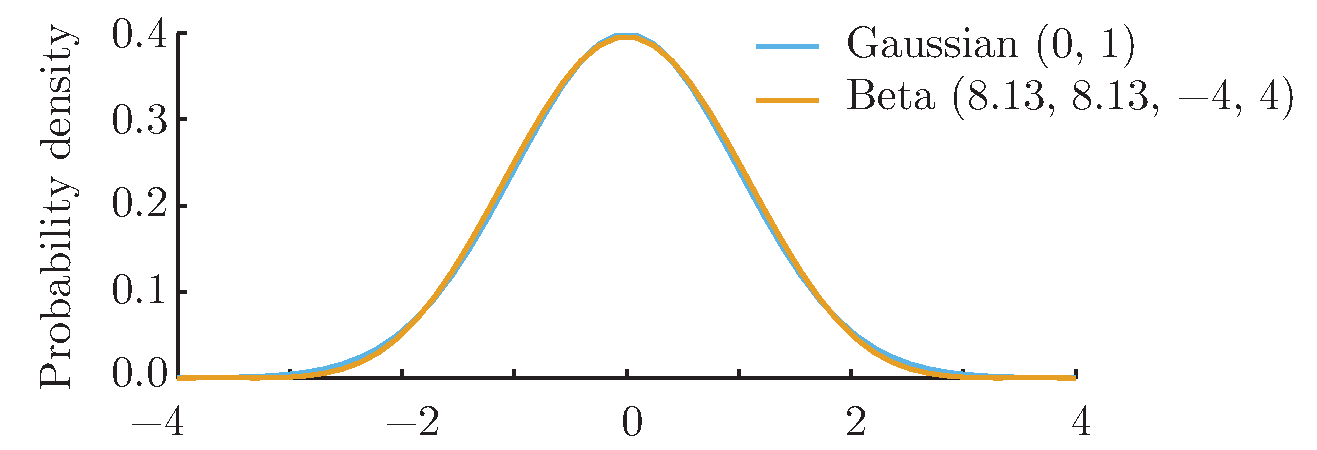
\includegraphics[width=0.9\ColumnWidth]{include/assets/beta-normal.pdf}
  \caption{The standard Gaussian distribution and a fitted beta distribution.}
  \flabel{beta-normal}
\end{figure}

The variability of $\Leff$ is split into global $\gLeff$ and local $\lLeff$ parts \cite{chandra2010, shen2009}.\footnote{Without loss of generality, $\gLeff$ can be treated as a composition of independent inter-lot, inter-wafer, and inter-die variations; likewise, $\lLeff$ can be treated as a composition of independent and dependent local variations.}
$\gLeff$ is assumed to be shared among all processing elements whereas each processing element has its own local parameter $\lLeff_i$.
Therefore, the effective channel length the $i$th processing element is modeled as follows:
\begin{equation} \elabel{leakage-partition}
  \Leff_i = \nLeff + \gLeff + \lLeff_i
\end{equation}
where $\nLeff$ is the nominal value of the effective channel length.
Hence, the uncertain parameters of the problem are
\begin{equation} \elabel{uncertain-parameters}
  \vU = \vec{\lLeff_1, \dotsc, \lLeff_\nprocs, \gLeff}.
\end{equation}

Global variations are typically assumed to be uncorrelated with respect to the local ones.
The latter, however, are known to have high spatial correlations, which we shall model using the following correlation function:
\begin{equation} \elabel{correlation-function}
  \fCorr(\vR_i, \vR_j) = \eta \; \fCorrSE(\vR_i, \vR_j) + (1 - \eta) \fCorrOU(\vR_i, \vR_j)
\end{equation}
where $\vR_i \in \real^2$ is the spatial location of the center of the $i$th processing element relative to the center of the die. The correlation function is a composition of two kernels:
\begin{align*}
  & \fCorrSE(\vR_i, \vR_j) = \exp\left(- \frac{\norm{\vR_i - \vR_j}^2}{\lCorrSE^2} \right) \text{ and} \\
  & \fCorrOU(\vR_i, \vR_j) = \exp\left(- \frac{\abs{\,\norm{\vR_i} - \norm{\vR_j}\,}}{\lCorrOU} \right),
\end{align*}
which are known as the squared-exponential and Ornstein-Uhlenbeck kernels, respectively.
$\eta \in [0, 1]$ is a weight coefficient balancing the kernels; $\lCorrSE$ and $\lCorrOU > 0$ are so-called length-scale parameters; and $\norm{\cdot}$ stands for the Euclidean distance.
The choice of the correlation function in \eref{correlation-function} is guided by the observations of the correlations induced by the fabrication process \cite{chandrakasan2001, friedberg2005, cheng2011}: $\fCorrSE$ imposes similarities between the spatial locations that are close to each other, and $\fCorrOU$ imposes similarities between the locations that are at the same distance from the center of the die (see also \cite{huang2009, ghanem1991, lee2013, bhardwaj2008, ghanta2006}).
The length-scale parameters $\lCorrSE$ and $\lCorrOU$ control the extend of these similarities, \ie, the range wherein the influence of one point on another is significant.

Although \eref{correlation-function} captures certain features inherent to the fabrication process, it is still an idealization.
In practice, it can be difficult to make a justifiable choice and tune such a formula, which is a prerequisite for the techniques in \sref{prior-work} based on the (continuous) KL decomposition.
A correlation matrix, on the other hand, can readily be estimated from measurements and, thus, is a more probable input to PTA.
Thus, we use \eref{correlation-function} with the only purpose of constructing a correlation matrix of $\{ \lLeff_i \}$.
For convenience, the resulting matrix is extended by one dimension to pack $\gLeff$ and $\{ \lLeff_i \}$ together.
In this case, the correlation matrix obtains one additional non-zero element on the diagonal.
Taking into account the variances of the variable, the final covariance matrix of the whole random vector $\vU$ (see \eref{uncertain-parameters}) is formed, which we denote by $\mCov_\vU$.

To conclude, an input to our analysis is the marginal distributions of the parameters $\vU$, which are beta distributions, and the corresponding covariance matrix $\mCov_\vU$.


\subsection{Parameter Preprocessing} \slabel{ie-uncertain-parameters}
The total dissipation of power is composed of two major parts: dynamic and leakage. The influence of process variation on the dynamic power is known to be negligibly small \cite{juan2011, juan2012, srivastava2010}; on the other hand, the variability of leakage is substantial, wherein the subthreshold current contributes the most \cite{juan2011, juan2012}. Hence, we focus on the subthreshold leakage and, more specifically, on the effective channel length denoted by $\Leff$. The variations of $\Leff$ are split into global (inter-die) and local (intra-die) parts \cite{chandra2010, juan2011, juan2012, srivastava2010, shen2009}. The global contribution is shared among all the processing elements and, therefore, is modeled as a single \rv\ $\gLeff(\o)$; furthermore, $\gLeff(\o)$ is typically assumed to be independent with respect to the local variations. The latter, however, are known to have high spatial correlations, which, due to particularities of the manufacturing process, often bear radial structures \cite{friedberg2005, cheng2011}. Therefore, as in \cite{ghanta2006}, we model the intra-die variations as a continuous-space stochastic process $\lLeff(r, \o)$ with the following radial covariance function \cite{ghanem1991}:
\begin{equation} \elabel{covariance-function}
  \fCov{\lLeff}{r_i, r_j} = e^{-|r_i - r_j|/\corrLength}
\end{equation}
where $r_i$ is the distance from the $i$th processing element to the center of the die, and $\corrLength$ is the correlation length. In words, the structure implies that the smaller the radial distance between two processing elements on the die, the more likely they are to have similar deviations of the effective channel length. Finally, it is generally accepted that the variations of the channel length have Gaussian distributions \cite{juan2011, juan2012, srivastava2010}. Therefore, we assume that the \rv\ $\gLeff(\o)$ as well as the process $\lLeff(r, \o)$ are Gaussian.

$\gLeff(\o)$ and $\lLeff(r, \o)$ form the input set of uncertain parameters $\vU(r, \o)$, which is to be processed in order to extract a finite set of mutually independent \rvs\ $\vZ(\o)$. Following the guidelines in \sref{uncertain-parameters}, Stage~1, the KL expansion suits the best in such a situation. A thorough elaboration on KL is out of the scope of this paper; however, the interested reader is referred to \aref{uncertain-parameters} where KL is applied to \eref{covariance-function}.


\subsection{Power Modeling} \slabel{ie-power-model}
The (total) power dissipation of the system with $\cores$ processing elements is given as the following sum:
\begin{equation} \elabel{power-model}
  \vP(\t, \o) = f_\dyn(\vP_\dyn(\t), \o) + f_\leak(\vTO(\t, \o), \o)
\end{equation}
where $f_\dyn, f_\leak: \real^\cores \times \outcomes \to \real^\cores$ model the dynamic and leakage power, respectively, as functions of the uncertain parameters $\vZ(\o)$. In addition, $f_\dyn$ depends on the nominal dynamic power $\vP_\dyn \in \real^\cores$, and the leakage part, $f_\leak$, depends on the operating temperature $\vTO \in \real^\cores$ due to the well-known non-linear interdependency between leakage and temperature, c.f. \cite{srivastava2010, liu2007}. We do not impose any further restrictions on $f_\dyn$ and $f_\leak$, and let the user to decide\footnote{One can easily find a dicent number of alternatives in the contemporary literature, for instance, follow the reference in \cite{srivastava2010}.}. Moreover, the functions are not required to have explicit mathematical formulations; they can be given as a `black box' as long as its inputs are in the set $\{ \vP_\dyn, \vTO, \vZ \}$.


\subsection{Thermal Modeling} \slabel{ie-thermal-model}
In this section, we provide additional details on the thermal model utilized by the proposed framework at \stage{3}\ described in \sref{thermal-model}.
We use the widespread model based on Fourier's heat equation \cite{skadron2004}, which, after a proper spacial discretization, leads to the following system:
\begin{subnumcases}{\elabel{fourier-system-original}}
  \mC \: \frac{d\,\vTI(\t)}{d\t} + \mG \: \vTI(\t) = \mM \: \vP(\t) \elabel{fourier-original} \\
  \vTO(\t) = \mM^T \vTI(\t) + \vTO_\amb
\end{subnumcases}
where the number of differential equations is equal to the number of thermal nodes denoted by $\nnodes$; $\mC \in \real^{\nnodes \times \nnodes}$ and $\mG \in \real^{\nnodes \times \nnodes}$ are a diagonal matrix of the thermal capacitance and a symmetric, positive-definite matrix of the thermal conductance, respectively; $\vTI \in \real^\nnodes$ is a vector of the difference between the temperature of the thermal nodes and the ambient temperature; $\vP \in \real^\nprocs$ and $\mM \in \real^{\nnodes \times \nprocs}$ are a vector of the power dissipation of the processing elements and its mapping to the thermal nodes, respectively; $\vTO \in \real^\nprocs$ is a vector of the temperature of the processing elements; and $\vTO_\amb \in \real^\nprocs$ is a vector of the ambient temperature.
$\mM$ distributes power across the thermal nodes.
Assuming that one processing element is mapped onto one thermal node, $\mM$ is filled in with zeros except for $\nprocs$ elements equal to unity that are located on the main diagonal.
For convenience, we perform an auxiliary transformation of the system in \eref{fourier-system-original} using \cite{ukhov2012}
\[
  \vS = \mC^\frac{1}{2} \vTI, \hspace{1em} \mA = -\mC^{-\frac{1}{2}} \mG \mC^{-\frac{1}{2}}, \hspace{1em} \text{and} \hspace{1em} \mB = \mC^{-\frac{1}{2}} \mM
\]
and obtain the system in \eref{fourier-system} where the coefficient matrix $\mA$ preserves the symmetry and positive-definiteness of $\mG$.
In general, the differential part in \eref{fourier-system-original} (and in \eref{fourier-system}) is nonlinear due to the source term $\vP(\t)$ since we do not make any assumptions about its structure (see the discussion in \sref{power-model}).
Therefore, there is no closed-form solution to the system.

The time intervals of the power and temperature profiles are assumed to be short enough such that the total power of a processing element can be approximated by a constant within one interval.
In this case, \eref{fourier-original} (and \eref{fourier-de}) is a system of linear differential equations that can be solved analytically.
The solution is as follows \cite{ukhov2012}:
\begin{equation} \elabel{ode-solution}
  \vS(\t) = \mCF(\t) \: \vS(0) + \mCS(\t) \: \vP(0)
\end{equation}
where $\t$ is restricted to one time interval, $\vP(0)$ is the power dissipation at the beginning of the time interval with respect to the corresponding temperature,
\begin{align*}
  & \mCF(\t) = e^{\mA \t} \in \real^{\nnodes \times \nnodes}, \hspace{1em} \text{and} \\
  & \mCS(\t) = \mA^{-1} (e^{\mA \t} - \mI) \: \mB \in \real^{\nnodes \times \nprocs}.
\end{align*}
The procedure is to be repeated for all $\nsteps$ time intervals starting from the initial temperature, which, without loss of generality, is assumed to be equal to the ambient temperature.
Note that, when the power profile is evenly sampled, the coefficient matrices $\mCF(\t)$ and $\mCS(\t)$ are constant and can be efficiently computed using the technique in \cite{ukhov2012}.
It is also worth noting that the described solution method belongs to the family of so-called exponential integrators, which have good stability properties; refer to \cite{hochbruck2010} for an overview.
Finally, taking into account $\vU$, we obtain \eref{recurrence}, operating on stochastic quantities.


\subsection{Surrogate Modeling} \slabel{ie-polynomial-chaos}
At \stage{4}, the independent \rvs, power model, and thermal model are fused together under the desired workload, $\profilePdyn$, to produce the corresponding stochastic power $\profileP{\o}$ and temperature $\profileT{\o}$ profiles. The obtained stochastic profiles are nothing more than two polynomials of $\Z_1(\o)$ and $\Z_2(\o)$ with time-dependent coefficients.

The construction of PC expansions is based on the Hermite basis (see \tref{askey}) as it was found to be optimal in situations involving Gaussian parameters \cite{xiu2010}.
A one-dimensional example of the basis is given in \fref{hermite} where the first six Hermite polynomials $\{ \pcb_i(\z) \}_{i = 1}^6$ are displayed.

In two dimensions, assuming a second-total-order PC expansion, the temperature at the $k$th moment of time is
\begin{align*}
  \vTO_k(\o) &= \pccs_{k1} + \pccs_{k2} \Z_1(\o) + \pccs_{k3} \Z_2(\o) + \pccs_{k4} \Z_1(\o) \Z_2(\o) \\
  & \qquad \qquad {} + \pccs_{k5} (\Z_1(\o)^2 - 1) + \pccs_{k6} (\Z_2(\o)^2 - 1)
\end{align*}
where $\pccs_{ki}$ are vectors with two elements corresponding to the two processors.

Once the basis has been chosen, we need to compute the corresponding coefficients, specifically, $\pcc{\vP}_i$ in \eref{pc-expansion}. As shown in \aref{polynomial-chaos}, the computation of $\pcc{\vP}_i$ involves multidimensional integration with respect to the \pdf\ of the \rvs\ $\vZ(\o)$.
In numerical analysis, this task is typically accomplished by virtue of a quadrature rule \cite{press2007}, which, loosely speaking, is a weighted summation over the integrand values computed at prescribed points. A natural choice of a quadrature rule when the weight function is a Gaussian \pdf\ is the Gauss-Hermite quadrature. Further details are given in \aref{gauss-quadrature}.

To summarize, we have completed four out of five stages of the proposed UQ framework depicted in \fref{algorithm}. The result is a light surrogate of the model in \eref{fourier-system}. At each moment of time, the surrogate is composed of two $\nprocs$-valued polynomials, one for power and one for temperature, that are defined in terms of $\nvars$ mutually independent \rvs; an example of such a polynomial is given in \eref{pc-k}. The constructed representation can be trivially analyzed to retrieve various statistics of the system in \eref{fourier-system}, and this is \stage{5}\ in \fref{algorithm}, which will be illustrated as a part of the next section.

\begin{figure}
  \centering
  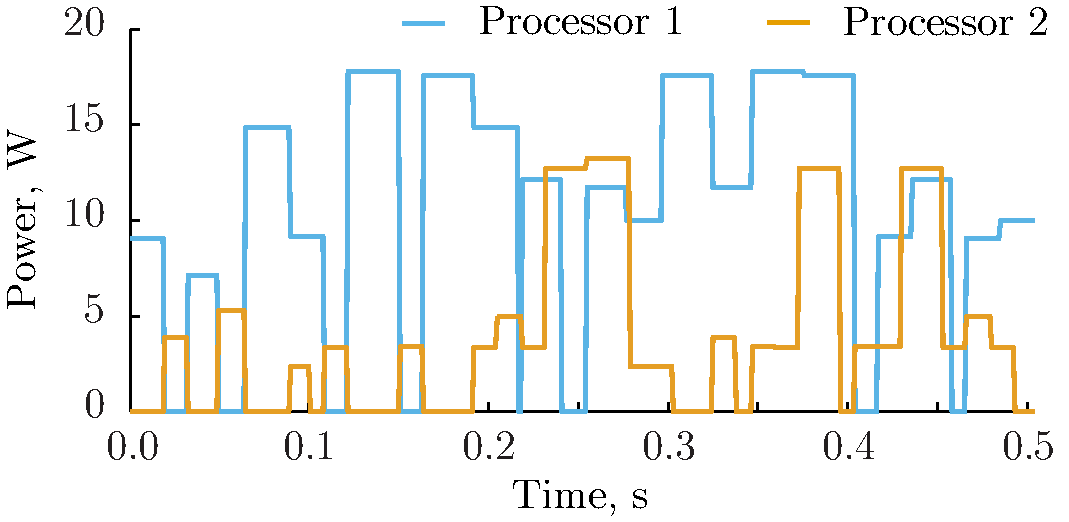
\includegraphics[width=1.00\columnwidth]{include/assets/application-power.pdf}
  \vspace{-0.5em}
  \caption{A dynamic power profile.}
  \flabel{application-power}
  \vspace{-0.5em}
\end{figure}

Assume that the dynamic power profile, $\profilePdyn$, corresponding to the considered workload is the one shown in \fref{application-power}.

\begin{figure}[bl]
  \vspace{-1.0em}
  \centering
  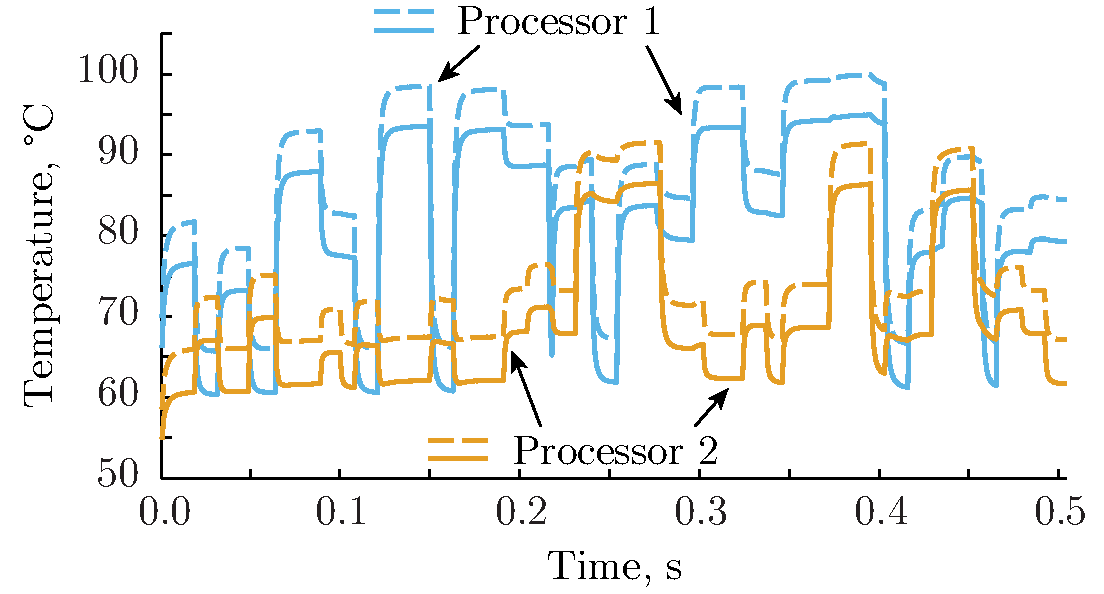
\includegraphics[width=0.90\columnwidth]{include/assets/application-temperature.pdf}
  \vspace{-0.5em}
  \caption{The expected temperature (the solid lines) and one standard deviation above it (the dashed lines).}
  \flabel{application-temperature}
\end{figure}

The expansion for power has the same structure but different coefficients.
Such a series might be shorter or longer depending on the accuracy requirements.
As we see, our surrogate model has a negligibly small computational cost to undertake UQ at \stage{5}: for any outcome of the uncertain parameters $\vZ(\o) \equiv \vZ$, we can easily compute the corresponding temperature by plugging $\vZ$ into the above equation; the same applies for power.
Thus, such characteristics as \cdfs\ and \pdfs\ (see \fref{motivation-pdf}) can be rigorously estimated. Furthermore, the expectation and variance at the $k$th moment of time are calculated as simply as
\[
  \oExp{\vTO_k(\o)} = \pccs_{k1} \hspace{1em} \text{and} \hspace{1em} \oVar{\vTO_k(\o)} = \sum_{i = 2}^{6} \pcn_i \: \pccs_{ki}^2
\]
where $\pcn_i$ are normalization constants, and the squaring should be understood element-wise.
For the nominal power profile $\profilePdyn$ depicted in \fref{application-power}, we obtain the corresponding stochastic temperature profile $\profileT{\o}$ and can observe, \eg, its expectation and standard deviation; they are plotted in \fref{application-temperature}.
The displayed curves closely match those obtained via MC simulations with $10^4$ samples; however, our method takes less than a second, on a personal laptop, while MC sampling takes more than a day, which we discuss in \sref{experimental-results}.


\subsection{Post-processing} \slabel{ie-post-processing}
\begin{figure}
  \centering
  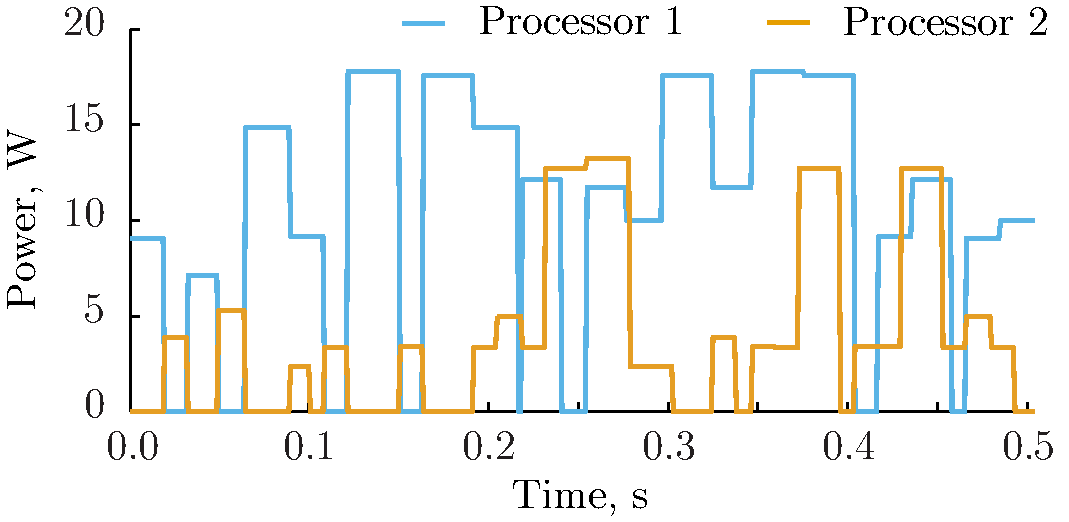
\includegraphics[width=1.00\columnwidth]{include/assets/application-power.pdf}
  \vspace{-0.5em}
  \caption{A dynamic power profile.}
  \flabel{application-power}
  \vspace{-0.5em}
\end{figure}

\begin{figure}[bl]
  \vspace{-1.0em}
  \centering
  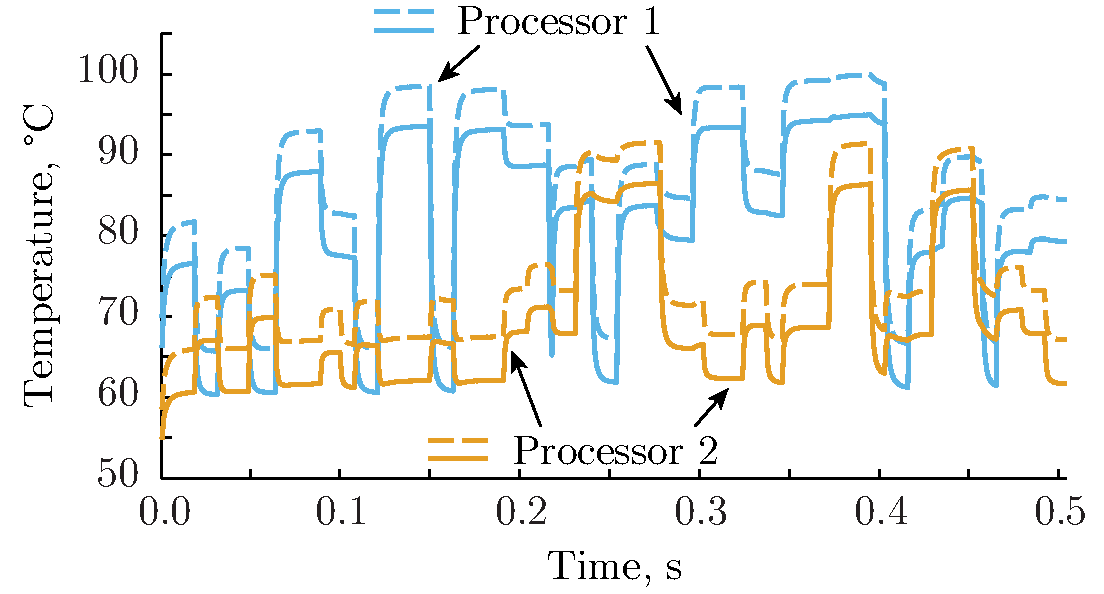
\includegraphics[width=0.90\columnwidth]{include/assets/application-temperature.pdf}
  \vspace{-0.5em}
  \caption{The expected temperature (the solid lines) and one standard deviation above it (the dashed lines).}
  \flabel{application-temperature}
\end{figure}

We turn to \stage{5}\ in \fref{algorithm}.
It can be seen in, for example, \eref{pc-example} that the surrogate model has a negligibly small computational cost at this stage: for any outcome of the uncertain parameters $\vZ(\o) \equiv \vZ$, we can easily compute the corresponding temperature by plugging in $\vZ$ into \eref{pc-example}; the same applies for power.
Consequently, the constructed representation can be trivially analyzed to retrieve various statistics of the system in \eref{fourier-system}.
Let us illustrate a few of them still retaining the example given in \eref{pc-example}.
Assume that the dynamic power profile, $\profilePdyn$, corresponding to the considered workload is the one shown in \fref{application-power}.
Having constructed the surrogate with respect to this profile, we can then rigorously estimate, say, the \pdf\ of temperature at some $k$th moment of time by sampling the surrogate and obtain curves similar to those shown \fref{experimental-results-pdf} (to be discussed in \sref{experimental-results}).
Furthermore, the expectation and variance of temperature are calculated simply as (see \eref{pc-moments})
\[
  \oExp{\vTO_k(\o)} = \pcc{\vTO}_{k1} \hspace{1em} \text{and} \hspace{1em} \oVar{\vTO_k(\o)} = \sum_{i = 2}^{6} \pcn_i \: \pcc{\vTO}_{ki}^2
\]
where $\pcn_i$ are normalization constants, and the squaring should be understood element-wise.
For the whole time span of the power profile $\profilePdyn$ depicted in \fref{application-power}, these quantities are plotted in \fref{application-temperature}.
The displayed curves closely match those obtained via MC simulations with $10^4$ samples; however, our method takes less than a second whilst MC sampling takes more than a day as we shall see next.



  \section{Experimental Results} \slabel{experimental-result}
  In this section, numerical results of the proposed framework for the illustrative example given in \sref{illustrative-example} are presented. All the experiments are implemented in MATLAB R2012a \cite{matlab} and conducted in \hostOS\ running on \hostHardware.

The effective channel length $\Leff$ is assumend to deviate by $5\%$ from the nominal value of $45$ nm where the global and local variations are equaly weighted \cite{juan2012}. Correlation matrices are computed according to \eref{correlation-matrix}, in which the correlation length $\corrLength$ is half the size of the die. The proposed framework is set up to construct Hermite PC expansions using non-intrusive Galerkin projections based on the Smolyak algorithm for multidimensional integration. In the model reduction technique, described in \sref{preprocessing-rvs}, the threshold parameter $\Lth$ is set to $0.99$, which makes the preserved eigenvalues capture $99\%$ of the variance of the data.

Dynamic power profiles involved in the experiments are based on simulations of synthetic applications on hypothetical platforms. Time steps of power and, consequently, temperature traces are set to one millisecond, i.e., $\dt_i = 10^{-3}$s, $\forall i$. The reference leakage current $I_\leak(\Leff, \T)$, obtained via SPICE simulations (see \sref{power-model-construction}), is scaled up to the power level of the processing elements in such a way that the leakage power accounts for about $40\%$ of the total power dissipation at high temperatures \cite{liu2007}. In order to construct equivalent thermal RC circuits, the temperature simulator HotSpot v5.02 \cite{hotspot} with default settings is employed. In this case, thermal packages are modeled with three layers, and the relation between the number of processing elements and the number of thermal nodes is given according to $\nodes = 4 \cores + 12$.

To assess the performance of our framework, we employ a Monte Carlo (MC) sampling technique. The MC approach consists in solving \eref{fourier-original} numerically using the Dormand-Prince method, which is based on the fourth- and fifth-order Runge-Kutta formulas \cite{press2007}. The leakage model for the MC sampling is the same as for the proposed framework except the fact that the model reduction is reasonably omitted.

\begin{table}
  \centering
  \caption{Normalized RMSE of expectation.}
  \vspace{-10pt}
  \begin{tabular}{crrrr}
    \toprule
    {} & $\err{\sExp}, \%$ & $\err{\sExp}, \%$ & $\err{\sExp}, \%$ & $\err{\sExp}, \%$ \\
    $\pcorder$ & $\mcsamples = 10^2$ & $\mcsamples = 10^3$ & $\mcsamples = 10^4$ & $\mcsamples = 10^5$ \\
    \midrule
    $1 $ & $0.13$ & $0.05$ & $0.21$ & $$ \\
    $2 $ & $0.23$ & $0.22$ & $0.02$ & $$ \\
    $3 $ & $0.26$ & $0.24$ & $0.01$ & $$ \\
    $4 $ & $0.26$ & $0.24$ & $0.01$ & $$ \\
    $5 $ & $0.26$ & $0.24$ & $0.01$ & $$ \\
%   $6 $ & $0.26$ & $0.24$ & $0.01$ & $$ \\
%   $7 $ & $0.26$ & $0.24$ & $0.01$ & $$ \\
%   $8 $ & $0.26$ & $0.24$ & $0.01$ & $$ \\
%   $9 $ & $0.26$ & $0.24$ & $0.01$ & $$ \\
%   $10$ & $0.26$ & $0.24$ & $0.01$ & $$ \\
    \bottomrule
  \end{tabular}
  \tlabel{accuracy-expectation}
  \vspace{-10pt}
\end{table}

\begin{table}
  \centering
  \caption{Normalized RMSE of variance.}
  \vspace{-10pt}
  \begin{tabular}{crrrr}
    \toprule
    {} & $\err{\sVar}, \%$ & $\err{\sVar}, \%$ & $\err{\sVar}, \%$ & $\err{\sVar}, \%$ \\
    $\pcorder$ & $\mcsamples = 10^2$ & $\mcsamples = 10^3$ & $\mcsamples = 10^4$ & $\mcsamples = 10^5$ \\
    \midrule
    $1 $ & $20.95$ & $30.39$ & $33.70$ & $$ \\
    $2 $ & $13.47$ & $ 6.66$ & $ 6.80$ & $$ \\
    $3 $ & $27.03$ & $ 7.85$ & $ 4.82$ & $$ \\
    $4 $ & $28.61$ & $ 8.87$ & $ 6.11$ & $$ \\
    $5 $ & $29.19$ & $ 9.26$ & $ 6.58$ & $$ \\
%   $6 $ & $29.53$ & $ 9.51$ & $ 6.88$ & $$ \\
%   $7 $ & $29.89$ & $ 9.76$ & $ 7.18$ & $$ \\
%   $8 $ & $30.23$ & $ 9.99$ & $ 7.46$ & $$ \\
%   $9 $ & $30.33$ & $10.05$ & $ 7.53$ & $$ \\
%   $10$ & $30.30$ & $10.03$ & $ 7.50$ & $$ \\
    \bottomrule
  \end{tabular}
  \tlabel{accuracy-variance}
  \vspace{-10pt}
\end{table}

The first set of experiments is aimed to identify the accuracy of both competitors and to find appropriate values of the polynomial order $\pcorder$ and the number of samples $\mcsamples$ for the PC expansion and MC sampling, respectively. The accuracy measure is chosen to be the normalized root mean square error (NRMSE) of expectation and variance, denoted by $\err{\sExp}$ and $\err{\sVar}$, respectively, of the resulting temperature traces. The comparison for a quad-core architecture with a dynamic power profile of $10^2$ steps is given in \tref{accuracy-expectation} for $\err{\sExp}$ and in \tref{accuracy-variance} for $\err{\sVar}$ where we vary $\pcorder$ from $1$ to $6$ and $\mcsamples$ from $10^2$ to $2 \times 10^4$. The veracity of the results increases from the top-left to the bottom-right corners of the tables, therefore, the last row can be viewed as an indicator of the MC error while the last column shows the error of the PC expansion. It can be seen that deviations of the expected value of both techniques are relatively small even for low precision requirements; for instance, $\err{\sExp}$ of the MC-based technique with $10^2$ samples is $2\%$, and $\err{\sExp}$ of the first-order PC expansion is only $0.81\%$. However, this is not the case with variance. The NRMSE for the MC approach starts from a large value of $186\%$ for $10^2$ samples and drops to $11\%$ for $10^3$ samples. The former is an outlier since $10^2$ samples are by far not sufficient for a MC technique. The later is a more realistic estimate, after which the MC sampling demonstrates its inherently slow rate of convergence \cite{xiu2009, maitre2010}. Even with $10^4$ samples, the different between the MC technique and the PC expansion is about $10\%$, and this difference is decreasing with the increase of $\mcsamples$, which means that the variance computed by the MC sampling converges to one of the PC expansion. Assuming that one can trust the statistics of $2 \times 10^4$ MC samples, we conclude that the error of the proposed framework is bounded by $1\%$ for expectation and by $5\%$ for variance for PC expansions of orders starting from four. Guided by the observations above, for the following experiments, we fix the number of samples $\mcsamples$ of the MC approach to $10^4$, which is typically consudered to be the lower bound, cf. \cite{xiu2009, bhardwaj2006}, and the polynomial order $\pcorder$ of the proposed framework to four.

\begin{table}
  \centering
  \caption{Scaling with the number of steps $\steps$.}
  \vspace{-10pt}
  \begin{tabular}{lrrr}
    \toprule
    $\steps$ & PC, seconds & MC, hours & Speedup, times \\
    \midrule
    $   10$ & $ 0.06$ & $   0.94$ & $5.89 \times 10^4$ \\
    $ 10^2$ & $ 0.07$ & $   3.60$ & $1.89 \times 10^5$ \\
    $ 10^3$ & $ 0.55$ & $  35.77$ & $2.34 \times 10^5$ \\
    $ 10^4$ & $ 5.47$ & $ 358.96$ & $2.36 \times 10^5$ \\
    $ 10^5$ & $54.39$ & $3643.42$ & $2.41 \times 10^5$ \\
    \bottomrule
  \end{tabular}
  \tlabel{scaling-steps}
  \vspace{-10pt}
\end{table}

Now, we investigate the scaling properties of the proposed framework with respect to the number of steps $\steps$ in the (nominal) dynamic power profile $\prof{\mP_\dyn}$, which is directly proportional to simulated time. The results for a quad-core architecture are given in \tref{scaling-steps}. Due to the long computation time demonstrated by the MC approach, its data for high values of $\steps$ are extrapolated based on a few samples. It can be seen that both methods scale linearly, which is expected. However, the proposed framework shows a superior performance being more around $10$--$40$ times faster than \emph{only one sample} of the MC technique.

\begin{table}
  \centering
  \caption{Scaling with the number of processing elements $\cores$.}
  \vspace{-10pt}
  \begin{tabular}{lcrrr}
    \toprule
    $\cores$ & $\vars$ & PC, seconds & MC, hours & Speedup, times \\
    \midrule
    $ 2$ & $2$ & $  0.39$ & $36.40$ & $3.37 \times 10^5$ \\
    $ 4$ & $2$ & $  0.37$ & $35.99$ & $3.51 \times 10^5$ \\
    $ 8$ & $4$ & $  1.87$ & $36.85$ & $7.08 \times 10^4$ \\
    $16$ & $4$ & $  3.55$ & $42.55$ & $4.32 \times 10^4$ \\
    $32$ & $7$ & $137.33$ & $45.21$ & $1.19 \times 10^3$ \\
    \bottomrule
  \end{tabular}
  \tlabel{scaling-cores}
  \vspace{-10pt}
\end{table}

The next parameter to exercise is the number of processing elements $\cores$ and, consequently, the number of stochastic dimensions $\vars$. In these experiments, the number of steps $\steps$ is constant and equal to $10^3$. The results are given in \tref{scaling-cores}. From the table, we can clearly see the well-known fact that the workload per one MC sample is independent of the number of stochastic dimensions \cite{maitre2010}. At the same time, we observe a polynomial growth \cite{heiss2008} of the PC expansion based on sparse grids, which is also predictable. However, even in high dimensions, the proposed framework significantly outperforms the MC sampling. For instance, to quantify a power profile with $10^3$ steps of a multiprocessor system with 32 cores, the MCS requires more than 35 hours whereas the proposed framework takes only 8 minutes. It should be noted separately that the number of samples of the MCS is constant in this setup; however, in order to maintain the same accuracy, the number of samples should be increased whenever $\vars$ is increased [?].


  \printbibliography
\end{document}
